\renewcommand*{\arraystretch}{1.5}
\noindent\begin{tabularx}{17cm}{|p{1.95cm}|X|}
	\hline
	number      & 12                                                          \\ \hline
	title       & Trending Posts                                                           \\ \hline
	\multicolumn{2}{|c|}{ 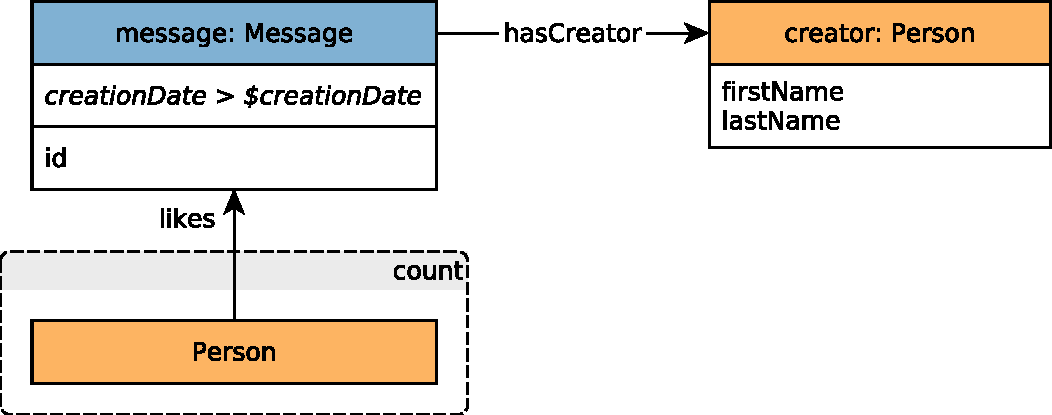
\includegraphics[scale=\patternscale,margin=0cm .2cm]{patterns/q12}} \\ \hline
	description & Find all Messages created after a given date, that received more than a
given number of likes.
 \\ \hline
	
	parameters  &
	\renewcommand*{\arraystretch}{1.0}
	\vspace{-1.8ex}{\begin{tabularx}{14.2cm}{|c|l|p{2cm}|Y|} \hline
	\cellcolor{black!70} \color{white} $\mathsf{ 1 }$ & \varname{creationDate} & \cellcolor{gray!20} \vartype{Date} & \\ \hline
	\cellcolor{black!70} \color{white} $\mathsf{ 2 }$ & \varname{likeThreshold} & \cellcolor{gray!20} \vartype{32bitInteger} & \\ 
	\end{tabularx}} \\ \hline
	result      &
	\renewcommand*{\arraystretch}{1.0}
	\vspace{-1.8ex}{\begin{tabularx}{14.2cm}{|c|l|p{2cm}|Y|} \hline
	\cellcolor{black!70} \color{white} $\mathsf{ 1 }$ & \varname{message.id} & \cellcolor{gray!20} \vartype{64bitInteger} & \\ \hline
	\cellcolor{black!70} \color{white} $\mathsf{ 2 }$ & \varname{message.creationDate} & \cellcolor{gray!20} \vartype{DateTime} & \\ \hline
	\cellcolor{black!70} \color{white} $\mathsf{ 3 }$ & \varname{creator.firstName} & \cellcolor{gray!20} \vartype{String} &The first name of the post's creator \\ \hline
	\cellcolor{black!70} \color{white} $\mathsf{ 4 }$ & \varname{creator.lastName} & \cellcolor{gray!20} \vartype{String} &The last name of the post's creator \\ \hline
	\cellcolor{black!70} \color{white} $\mathsf{ 5 }$ & \varname{likeCount} & \cellcolor{gray!20} \vartype{32bitInteger} &The number of Likes the Post received \\ 
	\end{tabularx}} \\ \hline
	sort        &
	\renewcommand*{\arraystretch}{1.0}
	\vspace{-1.8ex}{\begin{tabular}{|c|l|c|} \hline
	\cellcolor{black!70} \color{white} $\mathsf{ 1 }$ & \varname{likeCount} & \cellcolor{gray!20} $\desc$ \\ \hline
	\cellcolor{black!70} \color{white} $\mathsf{ 2 }$ & \varname{message.id} & \cellcolor{gray!20} $\asc$ \\ 
	\end{tabular}} \\ \hline
	limit       & 100                                                           \\ \hline
	choke points        &
	\multicolumn{1}{>{\raggedright}X|}{
		\chokepoint{1.2}, 
		\chokepoint{2.2}, 
		\chokepoint{3.1}, 
		\chokepoint{6.1}
		}\\ \hline
\end{tabularx}
\clearpage